\documentclass[journal,12pt,onecolumn]{IEEEtran}
\usepackage{cite}
 \usepackage{caption}
\usepackage{graphicx}
\usepackage{amsmath,amssymb,amsfonts,amsthm}
\usepackage{algorithmic}
\usepackage{graphicx}
\usepackage{textcomp}
\usepackage{xcolor}
\usepackage{txfonts}
\usepackage{listings}
\usepackage{enumitem}
\usepackage{mathtools}
\usepackage{gensymb}
\usepackage{comment}
\usepackage[breaklinks=true]{hyperref}
\usepackage{tkz-euclide} 
\usepackage{listings}
\usepackage{gvv}
%\def\inputGnumericTable{}                                 
\usepackage[latin1]{inputenc} 
\usetikzlibrary{arrows.meta, positioning}
\usepackage{xparse}
\usepackage{color}                                            
\usepackage{array}                                            
\usepackage{longtable}                                       
\usepackage{calc}                                             
\usepackage{multirow}
\usepackage{multicol}
\usepackage{hhline}                                           
\usepackage{ifthen}                                           
\usepackage{lscape}
\usepackage{tabularx}
\usepackage{array}
\usepackage{float}
\usepackage{amssymb}

\usepackage{float}
%\newcommand{\define}{\stackrel{\triangle}{=}}
\theoremstyle{remark}
\usepackage{circuitikz}
\captionsetup{justification=centering}
\usepackage{tikz}

\title{Matrices in Geometry 2.10.64}
\author{EE25BTECH11035 - Kushal B N}
\begin{document}
\vspace{3cm}
\maketitle
{\let\newpage\relax\maketitle}
\textbf{Question: }
The position vectors of the points $\vec{A}$, $\vec{B}$, $\vec{C}$ and $\vec{D}$ are $\brak{3\hat{i}-2\hat{j}-\hat{k}}$, $\brak{2\hat{i}+3\hat{j}-4\hat{k}}$, $\brak{-\hat{i}+\hat{j}+2\hat{k}}$ and $\brak{4\hat{i}+5\hat{j}+\lambda\hat{k}}$ respectively. If the points $\vec{A}$, $\vec{B}$, $\vec{C}$ and $\vec{D}$ lie on a plane, find the value of $\lambda$.
\bigskip

\textbf{Given: } \\
$\vec{A}\myvec{3\\-2\\-1}$, $\vec{B}\myvec{2\\3\\-4}$, $\vec{C}\myvec{-1\\1\\2}$ and $\vec{D}\myvec{4\\5\\\lambda}$.
\bigskip

\textbf{Solution: }\\

The general equation for a plane with normal vector $\vec{n}$ passing through point P is \\
\begin{equation}
    \vec{n}^{\top}\vec{P} = d
\end{equation}
So,
\begin{equation}
    \vec{n}^{\top}\vec{A} = d
\end{equation}

\begin{equation}
    \vec{n}^{\top}\vec{B} = d
\end{equation}

\begin{equation}
    \vec{n}^{\top}\vec{C} = d
\end{equation}

\begin{equation}
    \vec{n}^{\top}\vec{D} = d
\end{equation}

Forming direction vectors in the plane,

\begin{equation}
\vec{B} - \vec{A} = \myvec{-1\\5\\-3}
\end{equation}

\begin{equation}
\vec{C} - \vec{A} = \myvec{-4\\3\\3}
\end{equation}

Now, the normal vector will be orthogonal to both of these direction vectors, so that
\begin{equation}
    \brak{\vec{B} - \vec{A}}^{\top}\vec{n} = 0
\end{equation}

\begin{equation}
    \brak{\vec{C} - \vec{A}}^{\top}\vec{n} = 0
\end{equation}

Combining the above two equations,
\begin{equation}
    \myvec{\brak{\vec{B} - \vec{A}}^{\top}\\ \brak{\vec{C} - \vec{A}}^{\top}}\vec{n} = 0
\end{equation}

\begin{equation}
    \myvec{-1&5&-3\\-4&3&3}\vec{n} = \myvec{0\\0}
\end{equation}

Augmented matrix:
\begin{equation}
    \implies \myvec{-1&5&-3&|&0\\-4&3&3&|&0}
\end{equation}

\begin{equation}
    \myvec{-1&5&-3&|&0\\-4&3&3&|&0} \overset{R_2 \rightarrow R_2 - 4R_1}{\longrightarrow} \myvec{-1&5&-3&|&0\\0&-17&15&|&0}
\end{equation}

\begin{equation}
    \myvec{-1&5&-3&|&0\\0&-17&15&|&0} \overset{R_2 \rightarrow \frac{-1}{17}R_2}{\longrightarrow} \myvec{-1&5&-3&|&0\\0&1&\frac{-15}{17}&|&0}
\end{equation}

\begin{equation}
    \myvec{-1&5&-3&|&0\\0&1&\frac{-15}{17}&|&0} \overset{R_1 \rightarrow R_1 - 5R_2}{\longrightarrow} \myvec{-1&0&\frac{24}{17}&|&0\\0&1&\frac{-15}{17}&|&0}
\end{equation}

\begin{equation}
    \implies \vec{n} = \myvec{\frac{24}{17}\\ \frac{15}{17}\\ 1} t
\end{equation}

So we can take $t=17$ in order to get integer coefficients,
\begin{equation}
    \vec{n} = \myvec{24\\15\\17}
\end{equation}

Substituting this in (2),
\begin{equation}
    d = \myvec{24&15&17}\myvec{3\\-2\\-1} = 25
\end{equation}

So substituting for $\vec{D}$ and $d$ in the equation (5), we have
\begin{equation}
    \myvec{24&15&17}\myvec{4\\5\\\lambda} = 25
\end{equation}

\begin{equation}
    \implies \fbox{$\lambda = \frac{-146}{17}$}
\end{equation}

\textbf{Final Answer:}\\
The value of $\lambda$ is $\frac{-146}{17}$.

\begin{figure}[H]
    \centering
    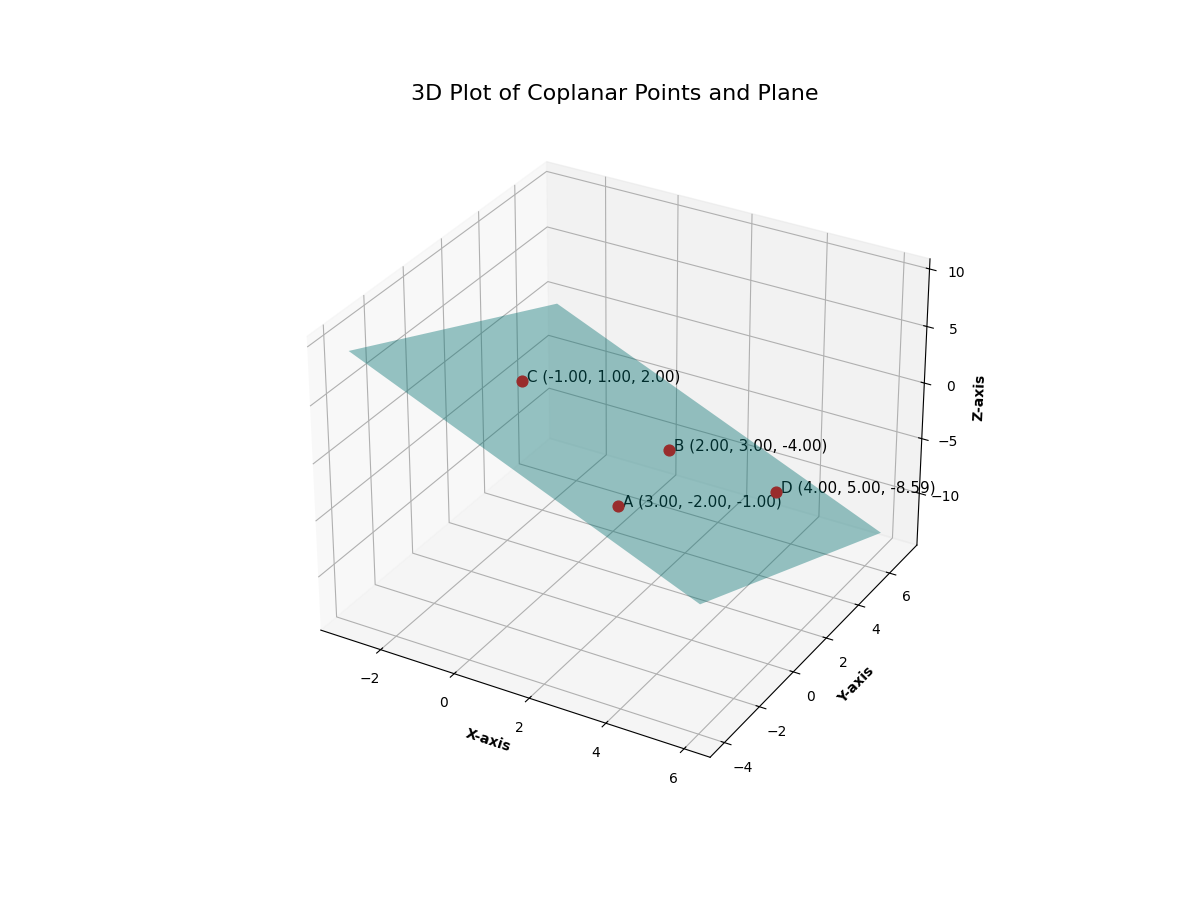
\includegraphics[width=1.05\columnwidth]{figs/2.png}
\end{figure}

\end{document}
